\documentclass[aspectratio=169,10pt]{beamer}
\usetheme{Madrid}
\usepackage[T1]{fontenc}
\usepackage{amsmath,amssymb}
\usepackage{booktabs}
\usepackage{tikz}
\usetikzlibrary{arrows.meta,positioning}
\setbeamertemplate{navigation symbols}{}
\setbeamertemplate{footline}{}
\setbeamerfont{block title}{size=\small}
\setbeamertemplate{itemize items}[circle]
\setlength{\tabcolsep}{5pt}

\title{Which Truth Does the Slide See?}
\subtitle{Auditing what pathology foundation models learn when IHC, mRNA and PAM50 disagree\\[3pt]\small Project Update}
\author{Aman Uniyal \and Aman Srivastava}
\institute{Topics in AI for Healthcare, IIIT Hyderabad\\[2pt]
  \footnotesize Base project: Kamineni -- Multimodal Breast Cancer Diagnostic \& Outcome Assistant}
\date{\today}

\begin{document}

%===================================================================
\begin{frame}
  \titlepage
\end{frame}

%===================================================================
\begin{frame}[t]{Proposal: Problem, Question \& Pipeline}
\footnotesize
\begin{columns}[T]
\begin{column}{0.48\textwidth}
\begin{block}{Clinical problem}
\begin{itemize}
  \item ER/PR/HER2 status drives therapy and is measured by \textbf{IHC}.
  \item IHC often disagrees with mRNA; on HER2 0 vs 1+ pathologists agree in only $\sim$26\% of cases.
  \item H\&E models learn whatever label they are given: \textbf{which biological truth do they track?}
\end{itemize}
\end{block}
\begin{alertblock}{Research question}
When IHC, RNA and PAM50 disagree, which one does an H\&E foundation model follow, and does it depend on the slide type?
\end{alertblock}
\end{column}
\begin{column}{0.48\textwidth}
\begin{block}{Five experiments (new evaluation, no new architecture)}
\begin{itemize}
  \item[\textbf{1a}] Is the IHC or the RNA label more predictable?
  \item[\textbf{1b}] On discordant cases, which side does the model take?
  \item[\textbf{1c}] Does it change from FFPE to frozen slides?
  \item[\textbf{1d}] Is HER2 0 vs 1+ visible in H\&E at all?
  \item[\textbf{1e}] Do two frozen slides of one tumour agree?
\end{itemize}
\end{block}
\end{column}
\end{columns}

\vspace{8pt}
\centering
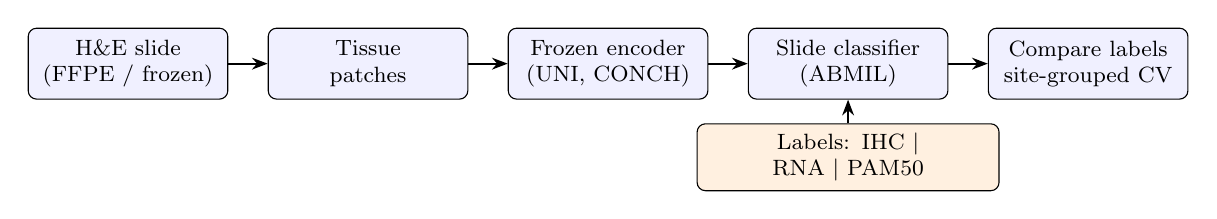
\begin{tikzpicture}[
  box/.style={draw, rounded corners=3pt, fill=blue!6, align=center, font=\footnotesize,
              text width=2.3cm, minimum height=0.9cm},
  lab/.style={draw, rounded corners=3pt, fill=orange!12, align=center, font=\footnotesize,
              text width=3.6cm, minimum height=0.6cm},
  arr/.style={-{Stealth[length=2mm]}, thick}, node distance=0.5cm]
  \node[box] (wsi) {H\&E slide\\(FFPE / frozen)};
  \node[box, right=of wsi] (patch) {Tissue\\patches};
  \node[box, right=of patch] (enc) {Frozen encoder\\(UNI, CONCH)};
  \node[box, right=of enc] (head) {Slide classifier\\(ABMIL)};
  \node[box, right=of head] (out) {Compare labels\\site-grouped CV};
  \node[lab, below=0.3cm of head] (labels) {Labels: IHC $\mid$ RNA $\mid$ PAM50};
  \draw[arr] (wsi) -- (patch);
  \draw[arr] (patch) -- (enc);
  \draw[arr] (enc) -- (head);
  \draw[arr] (head) -- (out);
  \draw[arr] (labels) -- (head);
\end{tikzpicture}
\end{frame}

%===================================================================
\begin{frame}[t]{Dataset: TCGA-BRCA}
\footnotesize
\begin{columns}[T]
\begin{column}{0.44\textwidth}
\begin{block}{Cohort}
\begin{itemize}
  \item 1,097 patients from 40 tissue-source sites (open access).
  \item Labels joined per patient from public metadata: IHC, RNA, PAM50, RPPA protein.
  \item Three slide types per patient:
\end{itemize}
\end{block}
\centering
\begin{tabular}{lrr}
\toprule
Slide type & Patients & Features \\
\midrule
FFPE diagnostic (DX) & 1,060 & public \\
Frozen top (TS) & 1,043 & ours \\
Frozen bottom (BS) & 427 & ours \\
\bottomrule
\end{tabular}
\end{column}
\begin{column}{0.52\textwidth}
\begin{block}{How often the ``truths'' disagree}
\centering
\begin{tabular}{llr}
\toprule
Marker & Compared & Discordant \\
\midrule
ER & IHC vs RNA & 5.5\% \\
PR & IHC vs RNA & 16.7\% \\
HER2 & IHC/FISH vs amplification & 10.8\% \\
\bottomrule
\end{tabular}
\end{block}
\begin{block}{Notes}
\begin{itemize}
  \item TCGA's HER2 field is noisy $\rightarrow$ we use a strict IHC/FISH rule.
  \item ER discordance is mostly ER-low tumours.
  \item \textbf{All five experiments are feasible} on public data (smallest: 1d, 57 vs 261 cases).
\end{itemize}
\end{block}
\end{column}
\end{columns}
\end{frame}

%===================================================================
\begin{frame}[t]{Baselines \& First Results}
\footnotesize
\textbf{Setup:} public TITAN slide embeddings (DX slides) $\rightarrow$ logistic regression; 5-fold CV, random vs site-grouped.
\vspace{4pt}
\begin{columns}[T]
\begin{column}{0.44\textwidth}
\centering
\begin{tabular}{lcc}
\toprule
H\&E $\rightarrow$ label (AUC) & Random & Site \\
\midrule
ER (IHC) & 0.89 & 0.89 \\
ER (RNA) & 0.94 & 0.92 \\
PR (IHC) & 0.80 & 0.79 \\
PR (RNA) & 0.80 & 0.79 \\
HER2 (clinical) & 0.73 & 0.67 \\
HER2 (amplification) & 0.76 & 0.76 \\
HER2 0 vs 1+ & 0.63 & \textbf{0.43} \\
Shuffled labels (control) & 0.43 & 0.46 \\
\bottomrule
\end{tabular}
\end{column}
\begin{column}{0.54\textwidth}
\begin{block}{1a: which label is more predictable?}
ER: \textbf{RNA beats IHC}, AUC 0.93 vs 0.88 ($\Delta$ +0.05, CI excludes 0). PR, HER2: no clear difference.
\end{block}
\begin{block}{1b: which side does the model take?}
On ER-discordant cases it sides with \textbf{RNA in 39/54} ($p$ = 0.0015); holds after removing borderline cases.
\end{block}
\begin{alertblock}{Site leakage}
Embeddings identify the hospital 82\% of the time; the HER2-low signal vanishes under site-grouped CV.
\end{alertblock}
\end{column}
\end{columns}
\end{frame}

%===================================================================
\begin{frame}[t]{Plan for the Next Week}
\footnotesize
\begin{columns}[T]
\begin{column}{0.32\textwidth}
\begin{block}{Stronger pipeline}
\begin{itemize}
  \item ABMIL on UNI patch features
  \item Repeated site-grouped CV with paired tests
  \item Robustness: RNA cut-offs, CONCH encoder
\end{itemize}
\end{block}
\end{column}
\begin{column}{0.32\textwidth}
\begin{block}{Experiments}
\begin{itemize}
  \item 1a, 1b for ER, PR, HER2 (+ protein label)
  \item 1d: HER2 0 vs 1+, compared with an mRNA model
  \item Start frozen slides for 1c, 1e
  \item Attention maps on discordant cases
\end{itemize}
\end{block}
\end{column}
\begin{column}{0.32\textwidth}
\begin{block}{Logistics}
\begin{itemize}
  \item Get UNI / CONCH access
  \item Download and encode 1,517 frozen slides
  \item Shared label table and fixed CV splits
\end{itemize}
\end{block}
\end{column}
\end{columns}

\vspace{10pt}
\centering
\begin{tabular}{lr}
\toprule
Compute on Ada (11\,GB GPUs) & Estimate \\
\midrule
Frozen-slide feature extraction & $\sim$1 day \\
Training all classifiers & 40--80 GPU-hours \\
Peak storage & $\sim$550\,GB of 1.8\,TB \\
\bottomrule
\end{tabular}
\end{frame}

\end{document}
